\chapter{Evaluaci\'on del programa original}
\label{ch:prev_work}

A continuaci\'on se ofrece una breve descripci\'on de la rutina original y se exponen los resultados de diferentes pruebas realizadas con ella, con la finalidad de medir su desempe\~no computacional en t\'erminos de tiempo de ejecuci\'on y uso de memoria, a la par de estudiar los resultados en el proceso de detecci\'on de las 93 supernovas halladas por HiTS durante la campa\~na del a\~no 2015.
\bigskip


\section{El programa}

La pipeline original est\'a estructurada por un proceso que puede dividirse en dos bloques: el primero est\'a destinado a buscar una supernova confirmada por HiTS (cuya coordenada es conocida) y encontrar nuevos candidatos; mientras que el segundo bloque, con la lista de coordenadas de nuevos candidatos, est\'a destinado a obtener la informaci\'on\footnote{Con informaci\'on se refiere a extraer muestras o estampillas desde las im\'agenes (de flujo, cient\'ifica, etc) como tambi\'en de las estructuras matriciales (matrices de estado, covarianza asociada, etc.) centradas en la coordernada del respectivo candidato.} de estos. El proceso general se inicializa con una instancia de \textsc{RunData}, la cual posee objetos de clases como \textsc{KalmanFilter} y \textsc{SNDetector} (con los cuales se configurar\'a la rutina), y con la cual se establecer\'an los par\'ametros a emplear a trav\'es de \textit{hard-coding}. Posterior a la configuraci\'on de par\'ametros se tiene una instancia de \textsc{FITSHandler}, para preparar las im\'agenes y el resto de archivos que ser\'an usados para el proceso iterativo que se describe a continuaci\'on:
\bigskip


\begin{enumerate}
\item \textbf{C\'alculo de flujo:} A partir de las im\'agenes cient\'ificas y de calibraci\'on se obtiene el flujo (en ADU\footnote{Analog-to-digital unit}) por p\'ixel y es registrado en una matriz (\texttt{numpy array}) en cada iteraci\'on. 
\item \textbf{Proceso de estimaci\'on con filtro de Kalman:} En este paso se realizan los procesos de predicci\'on y correcci\'on para obtener una nueva estimaci\'on. Se usa alguna instancia de uno de las clases \textsc{KalmanFilter} o \textsc{MaximumCorrentropyKalmanFilter} (en el programa original s\'olo est\'an implementados los filtros b\'asico y de m\'axima correntrop\'ia). 
\item \textbf{Detecci\'on de fuentes:} En este paso se estudia la idoneidad de los p\'ixeles tanto del flujo como de las estimaciones de los mismos (obtenidos con el filtro de Kalman) y del resto de las im\'agenes al momento de verificar una serie de criterios con los cuales estos se agrupar\'ian entre vecinos para formar candidatos (este proceso se realiza en \textsc{SNDetector}) (estos criterios son heredados en el futuro por la versi\'on refactorizada de este programa, en la clase \textsc{SourceFinder}). En la Figura \ref{fig:example}
se ejemplifica este proceso de agrupamiento.

\begin{figure}%
    \centering
    \subfloat[Los p\'ixeles son evaluados individualmente.]{{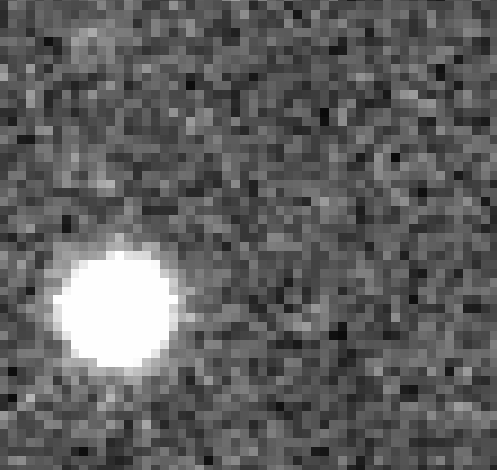
\includegraphics[width=5cm]{images/source.png} }}%
    \qquad
    \subfloat[Fuentes encontradas a partir de agrupamiento.]{{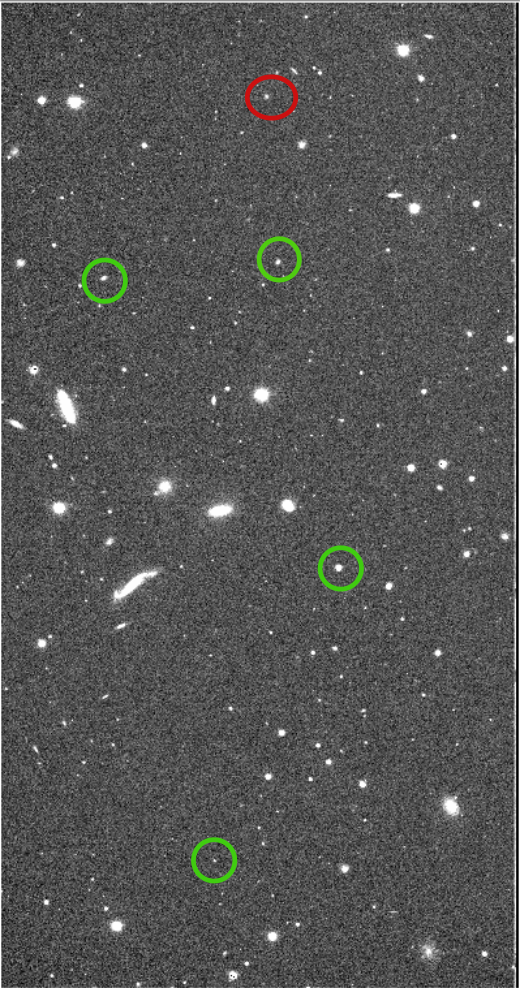
\includegraphics[width=5cm]{images/ccd_field.png} }}%
    \caption{La figura de la izquierda, corresponde a una muestra de una imagen cient\'ifica, en donde se logra observar sus p\'ixeles los cuales deben ser evaluados individualmente primero. Luego, en la figura derecha, se destaca en un c\'irculo rojo, la supernova conocida (SN34) y en c\'irculos verdes las fuentes candidatas a supernova, como resultado del proceso de agrupamiento de los p\'ixeles que satisfacen cierto conjunto de criterios.}%
    \label{fig:example}%
\end{figure}
 
\item \textbf{Actualizaci\'on de candidatos:} Revisa si hay nuevos candidatos a ser considerados. Los nuevos candidatos se registran en un arreglo (\texttt{numpy array}), mientras que los guarda la informaci\'on de la supernova conocida, en caso de encontrarse.
\end{enumerate}

Si en el proceso anterior se encuentran candidatos, se procede a repetir los pasos de obtenci\'on de flujos, estimaciones y filtrado de p\'ixeles. La diferencia est\'a en que en esta ocasi\'on se van guardando la informaci\'on de estos. El nuevo ciclo queda como sigue:

\begin{enumerate}

\item \textbf{Repetici\'on de los pasos anteriores 1-3}
\item \textbf{Guardado de resultados:} La informaci\'on de los nuevos candidatos encontrados previamente es guardada en la lista diccionarios \textit{obj} (variable de la clase \textsc{Observer}) y registrado en disco usando el formato NPZ (formato brindado por \textsc{Numpy} para comprimir datos).
\end{enumerate}


El diagrama de la Figura \ref{fig:des_sif} entrega una perspectiva general de la secuencia de pasos que realiza el programa. Sin embargo, nos encontramos con otro problema de implementaci\'on: la existencia de c\'odigo duplicado. Ya que ambos bloques est\'an repitiendo los mismos pasos salvo el \'ultimo en el que se diferencian en el registro de los resultados: en uno se guarda la informaci\'on de la supernova conocida (s\'olo si la detecta) y en el segundo, s\'olo si hay nuevos candidatos, guarda la informaci\'on de estos.
\bigskip

Cabe destacar que durante el proceso de estudio del programa original se encontr\'o que la lista de archivos, que debe ser procesada en orden cronol\'ogico, de acuerdo a la \'epoca (o fecha de observaci\'on), no est\'a siendo bien filtrada durante el proceso de selecci\'on de im\'agenes cient\'ificas en la clase \textsc{FITSHandler}, lo que puede involucrar imprecisiones en la detecci\'on de candidatos.
\bigskip


\begin{figure}[h!]
\centering
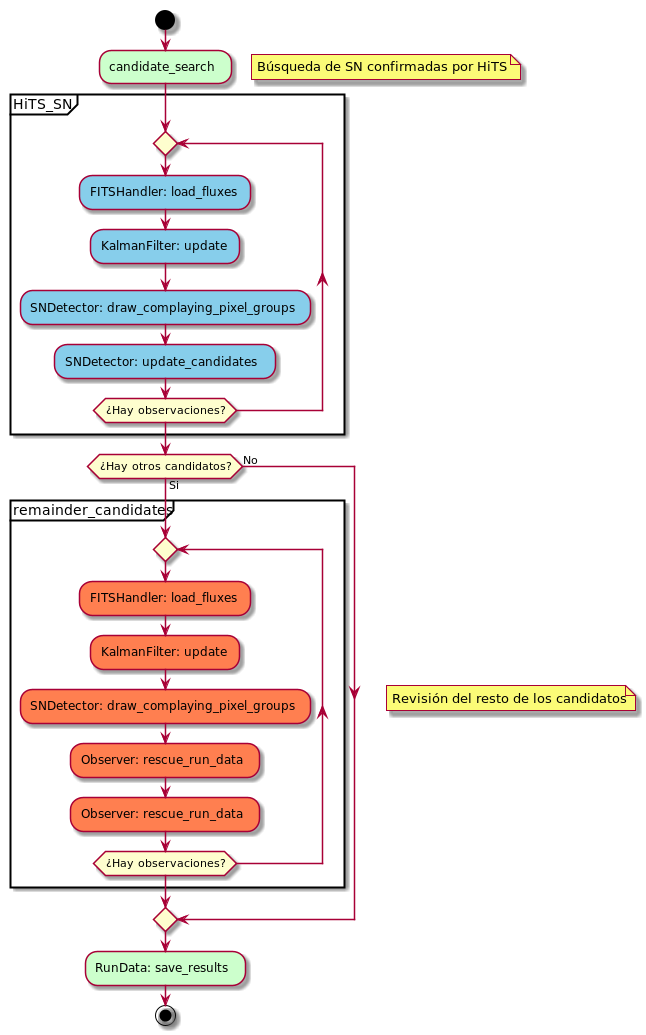
\includegraphics[scale=.5]{/home/paloma/Documents/Memoria/Code/sif2/sif_act}
\caption{Diagrama de flujo del programa original. Se aprec\'ian dos ciclos principales: el primero est\'a destinado a la b\'usqueda de una supernova en una coordenada dada y la revisi\'on de nuevos candidatos; y el segundo a la revisi\'on de la lista de candidatos encontrados en el primer bloque del proceso, para el guardado de la informaci\'on (extracci\'on de estampillas, desde cada matriz, centradas en sus coordenadas) de estos candidatos. Notar que hay pasos que se repiten en la realizaci\'on de ambos an\'alisis.}
\label{fig:des_sif}
\end{figure}

\section{Estructura de datos}
\label{des:struct}
Debido a la naturaleza de la informaci\'on de entrada (im\'agenes) se debe trabajar en p\'ixeles, por lo que la estructura de datos que representen las variables de estado debe considerar la dimensi\'on de las im\'agenes (teniendo en cuenta que por cada p\'ixel se debe modelar las variables de estado flujo y velocidad de flujo, y covarianza asociada). Debido a esto, en el trabajo de Pablo Huentelemu \cite{huentelemu} se dise\~naron \textit{hiperrect\'angulos} para modelar las variables de estado y covarianza de todos los p\'ixeles de una imagen. Los datasets contienen im\'agenes de dimensi\'on  $4094 \times 2046$. La Figura \ref{fig:data_scheme} muestra el esquema de sistema de matrices o \textit{hiperrect\'angulos} usada para representar el estado de cada p\'ixel y su respectiva covarianza.
\bigskip  

\begin{figure}
\centering
\includegraphics[scale=.35]{/home/paloma/Documents/Memoria/SVG/hola.png}
\caption{Esquema de las estructuras de datos usadas para la representaci\'on de las matrices de estados y de las matrices de covarianza de la relaci\'on entre el flujo ($x$) y la velocidad de flujo ($\dot{x}$) por cada p\'ixel, de una imagen de ancho $w$ y altura $h$. Para los conjuntos de datos, $w=2046$ y $h=4094$.}
\label{fig:data_scheme}
\end{figure}
\bigskip

\section{Pruebas}

Se realizaron dos tipos de prueba: la primera, orientada a medir tiempo de ejecuci\'on y uso de memoria principal, se llev\'o a cabo en un computador personal de 8 GB (DDR4) de RAM y una CPU de frecuencia 2.80 GHz sobre tres series de datos definidos por pares de CCD y campo en los que se sabe que hay una supernova. El segundo tipo de prueba se realiz\'o en Leftraru, pasando por algunas complicaciones relacionadas con el dise\~no del programa ya que el c\'odigo original contiene demasiadas l\'ineas con el comando \texttt{glob}\footnote{\url{https://docs.python.org/3.5/library/glob.html}} de Python (y una de las razones de porqu\'e se decidi\'o realizar el primer tipo de prueba en un computador personal), el cual lista reiteradamente el contenido de los directorios del \textit{home} del usuario lo que finalmente termina saturando el nodo destinado para el lanzamiento del programa si se tiene una gran cantidad de archivos. Este problema pudo resolverse eliminando documentos resultantes de pruebas iniciales. Cabe destacar que se adapt\'o el programa para Python 3.6, ya que originalmente estaba para 2.7 (ambos tipos de pruebas se realizaron para la versi\'on 3.6). En los dos tipos de prueba, se usaron los valores por defecto de los par\'ametros, estos son descritos en las secciones siguientes.
\bigskip


\subsection{Tiempo de ejecuci\'on}

El estudio del tiempo de ejecuci\'on del programa se realiz\'o usando la funci\'on \texttt{getrusage} de la librer\'ia \texttt{resource} de Python 3.6, midiendo el tiempo de usuario en segundos. Las mediciones se realizaron sobre tres conjuntos de datos, los cuales contienen alguna supernova detectada por HiTS, y que fueron seleccionados al azar: SN14, SN18 y  SN80. Cada uno de ellos comprende secuencias de 26, 23 y 18 observaciones, respectivamente. 
\bigskip

Las Tablas \ref{tab:t1} y \ref{tab:t2} muestran el tiempo en segundos que toma el proceso de detecci\'on de candidatos. Se destacan como procesos separados el reconocimiento de la supernova de HiTS y posteriormente, el proceso de estudio de los nuevos candidatos, respectivamente, empleando para ambos procesos el filtro b\'asico.  

\begin{table}[h!]
\centering
\caption{Resultados de tiempos de ejecuci\'on correspondientes a c\'alculo de flujo, estimaci\'on del filtro, agrupaci\'on de p\'ixeles y filtrado de los mismos durante el per\'iodo de reconocimiento de la supernova correspondiente. Para esta prueba se utiliz\'o el filtro de Kalman b\'asico. La \'ultima fila corresponde a la media por observaci\'on.}
\begin{tabular}{|l|r|r|r|r|}
\hline
\textbf{ID} & \textbf{C\'alc. Flujos [s]} & \textbf{Aplic. KF [s]} &  \textbf{Agrup. P\'ixeles [s]}  & \textbf{Actual. Candidatos [s]}\\ \hline \hline
SN14        & 293,91            & 24,90        &  68,30 & 0,02 \\ \hline
SN18            & 260,09             & 22,56         &  45,52  & 0,00\\ \hline
SN80            & 204,93             & 17,69         &   38,21 & 0,00 \\ \hline \hline
%Media & 303.08 &  26.23 & 37.83 & 0.01\\\hline 
$\bar{t}/Obs$ & 11,00 &  0,97 & 2,24 & 0,00\\\hline 
\end{tabular}
\label{tab:t1}
\end{table}

\begin{table}[h!]
\centering
\caption{Resultados de tiempos de ejecuci\'on correspondientes a c\'alculo de flujo, estimaci\'on de los filtros, agrupaci\'on de p\'ixeles y filtrado de los mismos durante el per\'iodo de estudio de los nuevos candidatos encontrados en el paso anterior. Para esta prueba se utiliz\'o el filtro de Kalman b\'asico. Se observa que para las dos \'ultimas supernovas los tiempos son cero ya que no se encontraron m\'as candidatos.}
\begin{tabular}{|l|r|r|r|r|}
\hline
\textbf{ID} & \textbf{C\'alc. Flujos [s]} & \textbf{Aplic. KF [s]} &  \textbf{Agrup. P\'ixeles [s]}  & \textbf{Guardar resultados [s]}\\ \hline \hline
SN14        & 303,18            & 27,28        &  72,34 & 0,02 \\ \hline
SN18            & 0,00             & 0,00         &  0,00  & 0,00\\ \hline
SN80            & 0,00             & 0,00         &   0.00 & 0,00 \\ \hline\hline 
%Media & 306.98 &  28.89 & 38.89  & 0.07\\\hline 
$\bar{t}/Obs$ & 11,66 &  1,05 & 2,78 & 0,00\\\hline 
\end{tabular}
\label{tab:t2}
\end{table}

Las Tablas \ref{tab:t3} y el \ref{tab:t4} describen el tiempo (en segundos) tomado tanto para el proceso de detecci\'on de la supernova de HiTS y el posterior procesamiento de posibles nuevos candidatos (en ese orden) usando el filtro de m\'axima correntrop\'ia.
\bigskip
 
\begin{table}[h!]
\centering
\caption{Resultados de tiempos de ejecuci\'on correspondientes a c\'alculo de flujo, estimaci\'on del filtro de Kalman, agrupaci\'on de p\'ixeles y filtrado de los mismos durante el per\'iodo de reconocimiento de la supernova correspondiente. Para esta prueba se utiliz\'o el filtro de Kalman de m\'axima correntrop\'ia.}
\begin{tabular}{|l|r|r|r|r|}
\hline
\textbf{ID} & \textbf{C\'alc. Flujos [s]} & \textbf{Aplic. KF [s]} &  \textbf{Agrup. P\'ixeles [s]}  & \textbf{Actual. Candidatos [s]}\\ \hline \hline
SN14        & 342,44            & 798,48        &  76,47 & 0,00 \\ \hline
SN18            & 273,64             & 566,89         &  47,96  & 0,00\\ \hline
SN80            & 210,68             & 420,12         &   36,05 & 0,00 \\ \hline \hline 
%Media & 309.32 & 638.48 &  37.07 & 0.01\\\hline
$\bar{t}/Obs. $& 12,25 & 26,23 & 2,34 & 0,00\\\hline 
\end{tabular}
\label{tab:t3}
\end{table}

\begin{table}[h!]
\centering
\caption{Resultados de tiempos de ejecuci\'on correspondientes a c\'alculo de flujo, estimaci\'on de los filtros, agrupaci\'on de p\'ixeles y filtrado de los mismos durante el per\'iodo de estudio de los nuevos candidatos encontrados en el paso anterior. Para esta prueba se utiliz\'o el filtro de Kalman de m\'axima correntrop\'ia. Se observa que para las dos \'ultimas supernovas los tiempos son cero ya que no se encontraron m\'as candidatos.}
\begin{tabular}{|l|r|r|r|r|}
\hline
\textbf{ID} & \textbf{C\'alc. Flujos [s]} & \textbf{Aplic. KF [s]} &  \textbf{Agrup. P\'ixeles [s]}  & \textbf{Guardar resultados [s]}\\ \hline \hline
SN14        & 307,64            & 680,65        &  65,67 & 0,02 \\ \hline
SN18            & 0,00             & 0,00         &  0,00  & 0,00\\ \hline
SN80            & 0,00             & 0,00         &   0,00 & 0,00 \\ \hline \hline
%Media & 306.71 & 634.09 &  36.34 & 0.05\\\hline
$\bar{t}/Obs. $& 11,83 & 26,18 & 2,53 & 0,00\\\hline  
\end{tabular}
\label{tab:t4}

\end{table}
\bigskip

La Tabla \ref{tab:t5} muestra el tiempo total comprendido por ambos subprocesos usando el filtro de Kalman b\'asico. Se destaca la diferencia del consumo de tiempo ante la ausencia y presencia de nuevos candidatos a supernova. Por otro lado, la Tabla \ref{tab:t6} muestran las mismas medidas de tiempo para el filtro de m\'axima correntrop\'ia. Se destaca el aumento considerable de tiempo al usar este \'ultimo filtro en relaci\'on al primero. 
  
\begin{table}[h!]
\centering
\caption{Tiempo de ejecuci\'on de los procesos de b\'usqueda de supernova de HiTS, revisi\'on de los candidatos encontrados y tiempo total comprendido por ambos procesos usando filtro de Kalman b\'asico. La \'ultima fila corresponde a tiempo total promedio por observaci\'on.}
\begin{tabular}{|l|r|r|r|}
\hline
\textbf{ID} & \textbf{B\'usqueda SN [s]} & \textbf{Revisi\'on candidatos[s]} & \textbf{Tiempo total [s]} \\ \hline
\hline
SN14 & 387,13 & 402,82 & 789,95 \\\hline
SN18 & 328,17 & 0,00 & 328,17\\\hline
SN80 & 260,83 & 0,00 & 260,83 \\\hline\hline
%Media & 367.15 & 374.83 & 741.98  \\\hline
 $\bar{t}/Obs. $& 14,55 & -- & --\\\hline 
\end{tabular}
\label{tab:t5}
\end{table}


\begin{table}[h!]
\centering
\caption{Tiempo de ejecuci\'on de los procesos de b\'usqueda de supernova de HiTS, revisi\'on de los candidatos encontrados y tiempo total comprendido por ambos procesos usando filtro de Kalman de m\'axima correntrop\'ia.}
\begin{tabular}{|l|r|r|r|}
\hline
\textbf{ID} & \textbf{B\'usqueda SN [s]} & \textbf{Revisi\'on candidatos [s]} & \textbf{Tiempo total [s]} \\ \hline
\hline
SN14 & 1217,39 & 1053,98 & 2068,80\\\hline
SN18 & 888,49 & 0,00 & 888,49\\\hline
SN80 & 666,85 & 0,00& 666,85\\\hline \hline
 $\bar{t}/Obs. $& 40,83 & -- & --\\\hline 
\end{tabular}
\label{tab:t6}
\end{table}

\subsection{Uso de memoria}

La memoria ocupada por el programa se midi\'o en t\'erminos de MiB (mebibytes) usando la librer\'ia \texttt{memory\_profiler}. Posteriormente las mediciones en la unidad previamente mencionada fueron pasadas a MB (megabytes) \footnote{$1MiB\simeq 1.049MB$ }.
\bigskip

La Figura \ref{fig:mem_kbf} muestra el comportamiento del uso de memoria principal (en t\'erminos de mebibytes) para los tres conjuntos de datos empleados, usando el filtro de Kalman b\'asico. Se distingue un uso m\'as intensivo (m\'aximo alcanzado) durante el proceso en que se usaron los datos de la SN14, la cual no s\'olo posee una secuencia de im\'agenes mayor (de 26) sino tambi\'en corresponde a aquella en donde se encontraron posibles nuevos candidatos. En la Tabla \ref{tab:mem1} se expone el m\'aximo consumo generado durante la ejecuci\'on de la pipeline empleando el filtro b\'asico.
\bigskip

\begin{figure}[h!]
\centering
\subfloat[Memoria ocupada en SN14]{\label{fig:kbf_14}{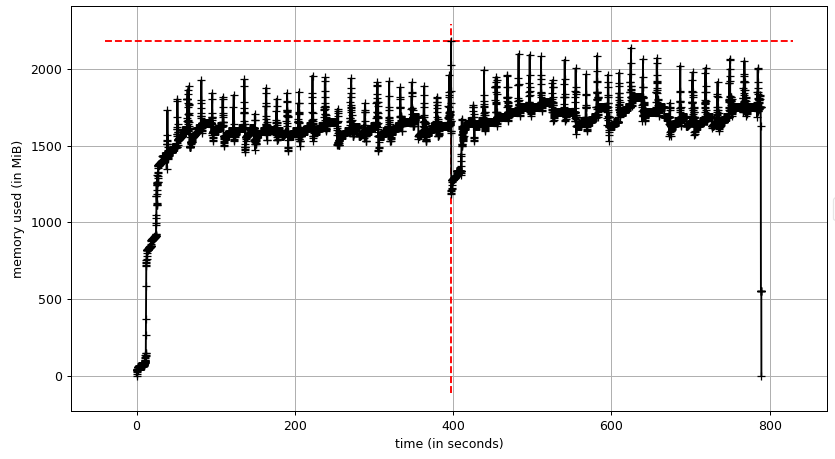
\includegraphics[width=0.5\textwidth]{images/results/sn14_00}}}\hfill
\subfloat[Memoria ocupada en SN18]{\label{fig:kbf_18}{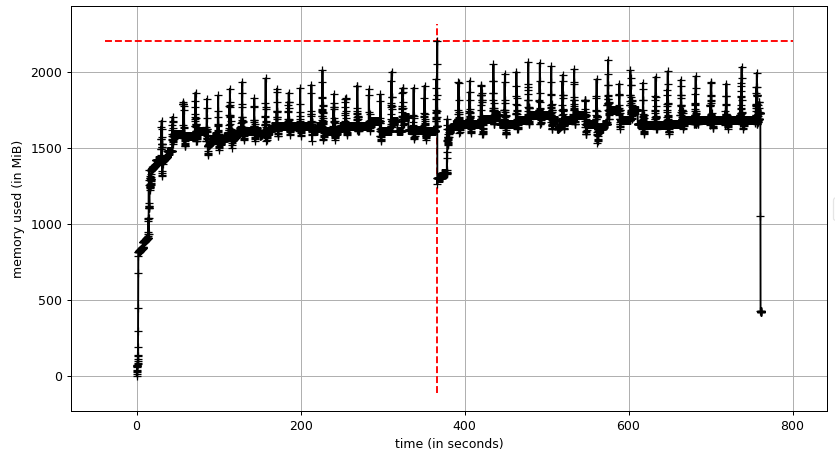
\includegraphics[width=0.5\textwidth]{images/results/sn18_00}}}\vfill
\subfloat[Memoria ocupada en SN80]{\label{fig:kbf_80}{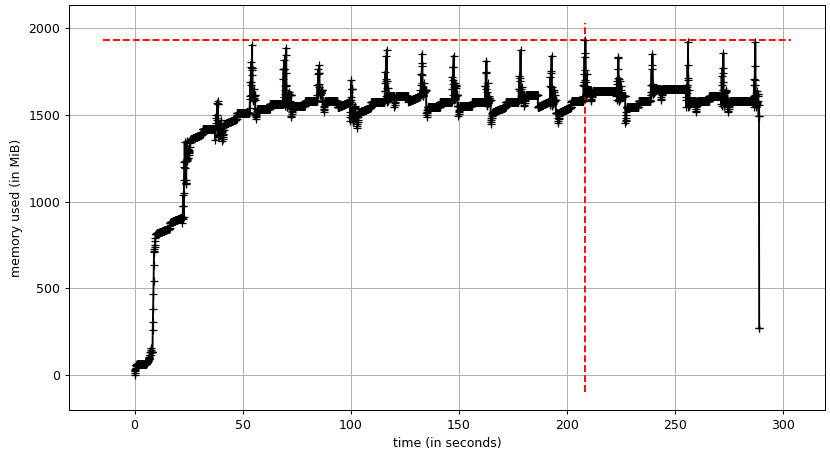
\includegraphics[width=0.5\textwidth]{images/results/sn80_00}}}
\caption{Comportamiento de la memoria (en mebibytes) durante la ejecuci\'on para los tres conjuntos de datos  de las supernovas SN14, SN18 y SN80, usando el filtro de Kalman b\'asico.}
\label{fig:mem_kbf}
\end{figure}

 
\begin{table}[h!]
\centering
\caption{Memoria principal (en unidades de MB) usada durante la ejecuci\'on del programa original con la versi\'on b\'asica del filtro de Kalman.}
\begin{tabular}{|l|r|}
\hline
\textbf{ID} & Memoria [MB]\\\hline\hline
SN14 & 2282,42\\\hline
SN18 & 2063,02\\\hline
SN80 & 2021,27\\\hline
\end{tabular}

\label{tab:mem1}
\end{table}


La Figura \ref{fig:mem_mcc} muestra el consumo de memoria (en mebibytes) para la ejecuci\'on del programa original para los tres conjuntos de datos, usando el filtro de m\'axima correntrop\'ia. Se destaca un comportamiento similar al obtenido usando el filtro b\'asico debido a  la detecci\'on de posibles candidatos con el conjunto de datos de la SN14. Por otro lado, se desprende un mayor consumo de parte de este filtro en relaci\'on a la versi\'on b\'asica. La Tabla \ref{tab:mem2} describe el consumo m\'aximo de memoria alcanzado con el uso del filtro de m\'axima correntrop\'ia.
\bigskip

\begin{figure}[h!]
\centering
\subfloat[Memoria ocupada en SN14]{\label{fig:mc_14}{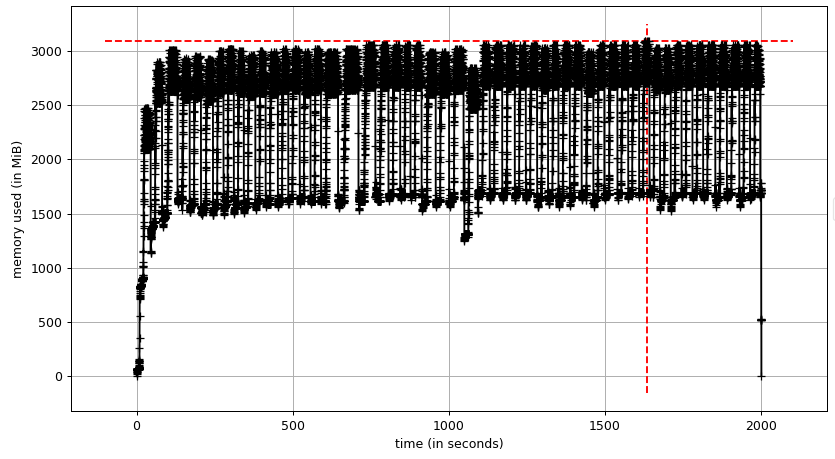
\includegraphics[width=0.5\textwidth]{images/results/sn14_01}}}\hfill
\subfloat[Memoria ocupada en SN18]{\label{fig:mc_18}{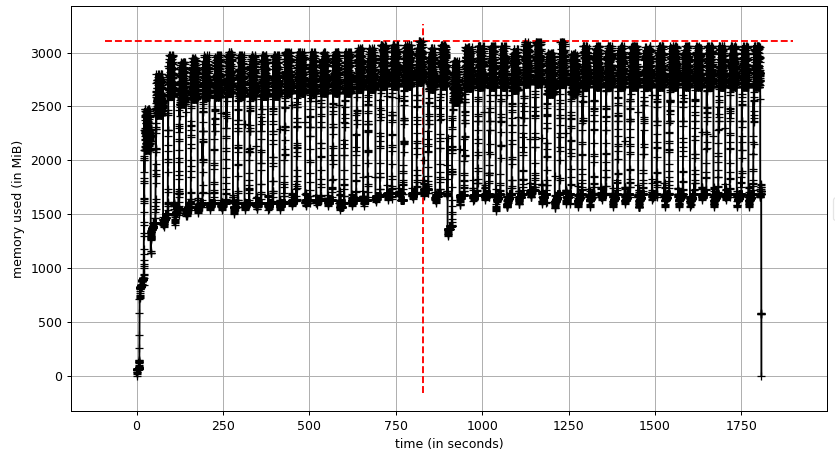
\includegraphics[width=0.5\textwidth]{images/results/sn18_01}}}\vfill
\subfloat[Memoria ocupada en SN80]{\label{fig:mc_80}{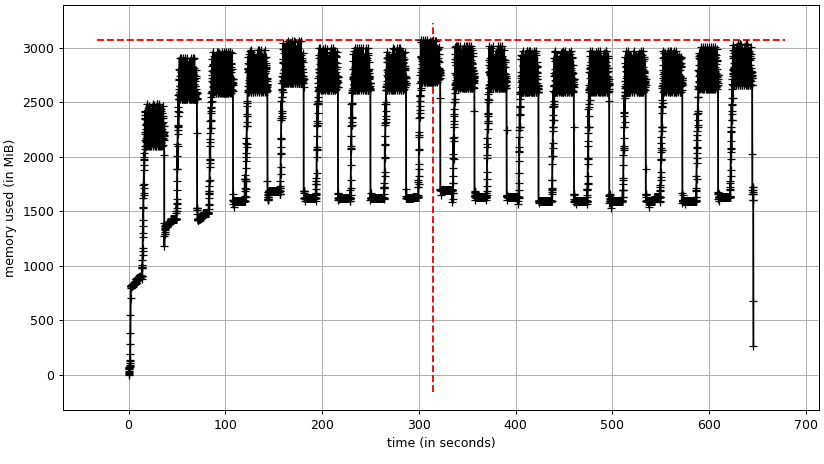
\includegraphics[width=0.5\textwidth]{images/results/sn80_01}}}
\caption{Comportamiento de la memoria (en mebibytes) durante la ejecuci\'on para los tres conjuntos de datos de las supernovas SN14, SN18 y SN80. En los tres lanzamientos se us\'o el filtro de Kalman de  m\'axima correntrop\'ia.}
\label{fig:mem_mcc}
\end{figure}


\begin{table}[h!]
\centering
\caption{Memoria principal (en unidades de MB) empleada durante la ejecuci\'on del programa original usando filtro de Kalman de m\'axima correntrop\'ia.}
\begin{tabular}{|l|r|}
\hline
\textbf{ID} & Memoria [MB]\\\hline\hline
SN14 & 3353,13\\\hline
SN18 & 3194,96\\\hline
SN80 & 3209,67\\\hline
\end{tabular}
\label{tab:mem2}
\end{table}

\subsection{Detecci\'on}
Se realizaron las pruebas de detecci\'on sobre los conjuntos de datos de las 93 supernovas en Leftraru durante el mes de febrero de 2019, usando los  umbrales de 200.0 para estimaci\'on de flujo y 50.0 para la velocidad de flujo. La Tabla \ref{tab:tpfn}, muestra el n\'umero de detecciones exitosas como verdaderos positivos (TP) as\'o como detecciones fallidas en t\'erminos de falsos negativos (FN) y falsos positivos (FP), y escenarios en donde la ejecuci\'on del programa fall\'o (por no encontrar archivos necesarios). 
\bigskip

\begin{table}[h!]
\centering
\caption{N\'umero de verdaderos positivos (TP), falsos negativos (FN) y falsos positivos (FP) (objetos no considerados por HiTS como supernova) encontrados usando cada uno de los filtros. La cuarta columna, \textbf{NaN} indica el n\'umero conjunto de datos que no se pudieron procesar por falta de alg\'un(os) archivo(s). No se observan diferencias sustanciales entre los resultados de cada filtro. Con el filtro de m\'axima correntrop\'ia se encontr\'o un falso positivo menos.}
\begin{tabular}{|l|r|r|r|r|}
\hline
\textbf{Filtro} & \textbf{TP} & \textbf{FN} & \textbf{FP}  & \textbf{NaN}\\ \hline
Básico          & 33          & 57         & 53 & 3 \\ \hline
MCC             & 33          & 57         & 52 & 3 \\ \hline
\end{tabular}
\label{tab:tpfn}
\end{table}

Para los par\'ametros usados (p\'arrafo anterior) se obtienen resultados id\'enticos para ambos filtros en t\'erminos de cantidad de supernovas detectadas. En ambos casos se detectaron 33, sin embargo existe una leve diferencia en la cantidad de falsos positivos: el programa, usando el filtro de m\'axima correntrop\'ia encuentra un falso positivo menos que al usar el filtro b\'asico. Para ambos casos, tres secuencias de supernovas no pudieron ser procesadas (cuyos resultados fueron etiquetados como \textit{NaN}) debido a la falta de im\'agenes de invarianza inversa (esenciales para el c\'alculo de flujo). Cabe destacar que para estos experimentos no se us\'o la optimizaci\'on de Silverman, ya que su implementaci\'on estaba incompleta.  %, ya que para tres supernovas (de las 93 y \'ultimas en la lista) no se encontraron las im\'agenes de invarianza inversa.
\bigskip

%Se debe se\~nalar que durante las primeras pruebas con el programa original, en su versi\'on para Python 2.7, se detectaban 33 supernovas de las 93, no obstante al actualizar el c\'odigo para una versi\'on compatible con Python 3.6, se obtiene un mejor resultado para los dos tipos de filtros, detect\'andose dos supernovas m\'as. Se piensa que esto puede deberse a la actualizaci\'on de la librer\'ia \textsc{PyMorph}\footnote{\url{https://pythonhosted.org/pymorph/}} por \textsc{Mahotas}\footnote{\url{https://mahotas.readthedocs.io/en/latest/}} (ambas librer\'ias desarrolladas por el mismo autor, Luis P. Coelho\footnote{\url{https://github.com/luispedro}}). 
%\bigskip

\subsection{Observaciones}
A partir de los resultados obtenidos, se procedi\'o a estudiar las curvas de luz (cuyo flujo se mide ADU) \footnote{analog-to-digital unit} considerando escenarios en donde supernovas conocidas son detectadas por el programa (con ambos filtros) (Figura \ref{fig:sns_found}) y donde no ocurre (Figura \ref{fig:sns_not_found}). 

\begin{figure}[h!]
\centering
\includegraphics[scale=0.5]{/home/paloma/Documents/Memoria/Background/light_curves/found0.png}
\caption{Curvas de luz (flujo en ADU vs tiempo en MJD) de 16 supernovas detectadas tanto por el filtro de Kalman b\'asico como el de m\'axima correntrop\'ia. Esta figura corresponde a un an\'alisis exploratorio de resultados obtenidos a trav\'es de m\'etodos fotom\'etricos tradicionales (no por filtros de Kalman), y est\'an disponibles junto a la base de datos de HiTS \cite{hits}.}
\label{fig:sns_found}
\end{figure}

\begin{figure}[h!]
\centering
\includegraphics[scale=0.5]{/home/paloma/Documents/Memoria/Background/light_curves/not_found0.png}
\caption{Curvas de luz (flujo en ADU vs tiempo en MJD) de 16 supernovas no detectadas ni por el filtro de Kalman b\'asico ni por el de de m\'axima correntrop\'ia. Esta figura corresponde a un an\'alisis exploratorio de resultados obtenidos a trav\'es de m\'etodos fotom\'etricos tradicionales (no por filtros de Kalman), y est\'an disponibles junto a la base de datos de HiTS \cite{hits}. Se aprecia el r\'apido crecimiento en la luminosidad de una de ellas.}
\label{fig:sns_not_found}
\end{figure}

En la Figura \ref{fig:sns_found} se observa, a grandes rasgos, la presencia de una etapa de crecimiento en el flujo de los objetos (supernovas), coincidiendo con el per\'iodo de alta cadencia mencionado en el cap\'itulo anterior (Cap\'itulo \ref{ch:background}, subsecci\'on \ref{ssec:data}), mientras que por el contrario en la imagen \ref{fig:sns_not_found} el comportamiento de los flujos es m\'as bien irregular y no se distinguen etapas de crecimiento constante. Hay que mencionar que el algoritmo principal, aquel cuya tarea es la de filtrar y agrupar p\'ixeles bajo criterios de descarte (implementado en \textsc{SNDetector}), emplea un sistema de \textit{alerta} interno con el cual se gatilla una detecci\'on cuando un grupo determinado de p\'ixeles satisface una serie de requisitos durante cuatro \'epocas consecutivas. Para gatillar esta alerta, uno de los requisitos que debe cumplir un grupo de p\'ixeles para considerarse candidato a supernova es el crecimiento continuo de los flujos por p\'ixel. Si ocurre un descenso entonces el grupo es inmediatamente descartado.  
%Al estudiar los periodos de las detecciones de cada uno de los conjuntos de datos de las supernovas de HiTS, para ambos filtros, se obtiene que no hay diferencias en la \'epoca en que se realiza (es decir misma hora o MJD). Ver Ap\'endice, secci\'on \ref{ap:tab1}. 
\bigskip

Las Figuras \ref{fig:orig_det_snL} y \ref{fig:orig_det_snaa} muestran dos casos del intervalo de tiempo en que se realizan detecciones exitosas usando ambas implementaciones de los filtros del programa original (ver Ap\'endice, secci\'on \ref{ap:tab1} para conocer lista completa de fechas de detecciones).
\bigskip

\begin{figure}[h!]
\centering
\includegraphics[scale=0.35]{/home/paloma/Documents/Memoria/SVG/hits_snL.png}
\caption{Curva de luz (en ADU vs MJD) de supernova registrada en el CCD N27, campo 34. La detecci\'on realizada por los filtros b\'asico y de m\'axima correntrop\'ia se realiz\'o en el MJD 57072.214 (\'epoca u observaci\'on 7 de 18). }
\label{fig:orig_det_snL}
\end{figure}


\begin{figure}[h!]
\centering
\includegraphics[scale=0.35]{/home/paloma/Documents/Memoria/SVG/hits_snaa.png}
\caption{Curva de luz supernova observada en el CCD S5, campo 21. Ambos filtros detectaron la supernova en el MJD 57077.166 (\'epoca u observaci\'on 23 de 27).}
\label{fig:orig_det_snaa}
\end{figure}
\bigskip

\subsubsection{Falsos positivos}
Para reconocer falsos positivos se requiere contar con una herramienta externa de visualizaci\'on o de \textit{machine learning}, por ejemplo, usando un clasificador de conjuntos de p\'ixeles que eval\'ue la probabilidad de que se trata efectivamente de una supernova joven. Esto se debe a que existen variados objetos como estrellas variables o \textit{artefactos} que corresponden a zonas ruidosas de la imagen  cient\'ifica (en particular, bordes) y pueden proveer valores alterados de flujo lo que en algunos casos puede conllevar a la detecci\'on de falsos positivos.
\bigskip

Una forma de poder estudiar un falso positivo es a trav\'es de la visualizaci\'on de su espacio de fase y la obtenci\'on de la entrop\'ia de la curva.